\chapter{Auswertung, Fehlerrechnung und Diskussion der Messergebnisse}
\section{Aufgabe 1: Einfluss der Spitzengeometrie}
Der Einfluss der Spitzengeometrie wurde bereits in Kapitel \ref{chap:aufloesung} behandelt. Im Rahmen dieser Aufgabe sollen die Scanlinien zu den in Abbildung \ref{fig:faelle} angegebenen Fällen aufgezeigt werden. Diese sind in Abbildung \ref{fig:scanlinien} sichtbar. 
\begin{figure}[H]
    \centering
    \includegraphics[width=110mm,scale=0.5]{Rasterkraftmikroskop/include/fälle.png}
    \caption{Zu behandelnde Fälle} 
    \label{fig:faelle}
\end{figure}

\begin{figure}[H]
    \centering
    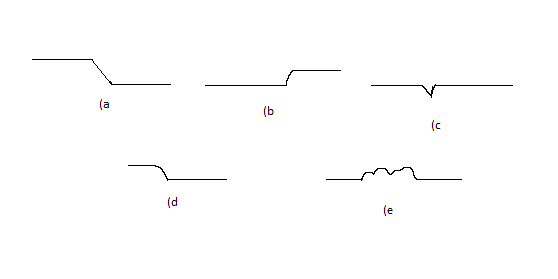
\includegraphics[width=110mm,scale=0.5]{Rasterkraftmikroskop/include/scanlinien.png}
    \caption{Die entstehenden Scanlinien} 
    \label{fig:scanlinien}
\end{figure}
Es ist ersichtlich, das die Geometrie der Spitze großen Einfluss auf die Scanlinien hat. Merkmale der Probenoberfläche können nur korrekt abgebildet werden, wenn Ausmaße größer als die der Spitze sind. So kann zum Beispiel Fall c nicht richtig abgebildet werden. Spitzenartefakte in der Scanlinie lassen sich durch Änderung der Scanrichtung einfacher identifizieren, jedoch ist eine genaue Zuordnung meistens nicht möglich.   

\section{Aufgabe 2: Einfluss des Spitzenradius}
Unter der Vorraussetzung, das sowohl Spitze als auch Topographiedetail Halbkugeln mit Radius $R$ bzw. $r$ sind, lässt sich über den Satz des Pythagoras die folgende Gleichung aufstellen
$$R^2 + R_mess^2 = (R+r)^2$$
wobei $R_mess$ der gemessene Radius des Topographiedetail ist. 
Woraus folgt
$$R = \frac{R_mess^2 - r^2}{2r}$$
Will man nun eine Vergrößerung des Messergebnisses von höchstens \SI{10}{\%}, setzt man für $R_mess = 1,1 r$ ein. 
Damit ergibt sich ein Detailradius von
$R = 0.105r, r = 9.524R$
Das Detail muss somit einen Radius von mindestens $9.524\cdot R$ haben, damit das Messergebnis um weniger als \SI{10}{\%} vergrößert wird.


\section{Aufgabe 3: Federkonstante des Cantilevers}
Die Federkonstante des Cantilevers kann mithilfe der Gleichung $$c_n = \frac{E\cdot w\cdot t^2}{4 \cdot l^3}$$ bestimmen. Dabei ist $E$ das Elastizitätsmodul, $w$, $t$ und $l$ die Dimensionen des Cantilevers. 
Mit den gegebenen Daten $E = \SI{1.69 }{\cdot 10^{11}\frac{N}{m^2}}, l = \SI{350 \pm 5}{\mu m}, w = \SI{35 \pm 3}{\mu m}, t = \SI{1 \pm 0.3}{\mu m}$ und gausscher Fehlerfortpflanzung ergibt sich die Federkonstante zu
$$c_n = \SI{0.03 \pm 0.02}{\frac{N}{m}}$$
was mit dem im Datenblatt gegebenen Wert übereinstimmt. 